\documentclass[10pt,a4paper]{article}
\usepackage[utf8]{inputenc}
\usepackage[english]{babel}
\usepackage[T1]{fontenc}
\usepackage{amsmath}
\usepackage{amsfonts}
\usepackage{amssymb}
\usepackage{makeidx}
\usepackage{graphicx}
\usepackage{fourier}
\usepackage{listings}
\usepackage{color}
\usepackage{hyperref}
\usepackage[left=2cm,right=2cm,top=2cm,bottom=2cm]{geometry}
\author{Johannes Scheller, Vincent Noculak, Lukas Powalla, Richard Asbah}
\title{Computational Physics - Project 4}

\lstset{language=C++,
	keywordstyle=\bfseries\color{blue},
	commentstyle=\itshape\color{red},
	stringstyle=\color{green},
	identifierstyle=\bfseries,
	frame=single}
\begin{document}

\maketitle
\newpage
\tableofcontents
\newpage


\section{Results}

%	e part:

In figure \ref{e_all}, \ref{absm_all}, \ref{chi_all} and \ref{cv_all}, the expectation values $<E>$ and $<|M|>$, the specific heat $C_V$ and the susceptibility $\chi$ for lattice sizes $L = 20, 40, 60, 80$ can be seen as functions of $T$ close to the critical temperature. It is the easiest to estimate the critical temperature by looking at figure \ref{cv_all}, because it is at the temperature where $C_V$ is the highest. In figure \ref{cv2040} and \ref{cv6080} we increased the number of Monte Carlo cycles and decreased the temperature step length and interval to determine the temperature of the maximum of $C_V$ more precisely. In table \ref{tc} the measured critical temperatures can be seen. While it is possible to measure $T_C$ even more precisely by increasing the Monte Carlo cycles and decreasing the Temperature step length, it is not possible aim at any precision, due to the quickly increasing calculation time. 
In figure \ref{chi_all} we can see that near $T_C$ the measured values for the susceptibility are very unstable. At $T_C$ it peak down to a very low value and then increases again to go against zero. In figure \ref{e_all} is can be observed that at $T_C$ the slope of the curve $<E(T)>$ starts to decrease again. As already mentioned in figure \ref{cv_all} we can clearly see a peak of the graph at $T_C$. In this graph it can also be seen, that the critical temperature decreases with bigger lattice sizes. 

Figure \ref{absm_all} shows, that while $<|M|>$ stays nearly stable at a non-zero value and decreases very slow for temperatures much smaller than $T_C$, near the critical temperature it decreases quickly and goes against zero. This is a shows that a phase transition is taking place. For a temperature lower than $T_C$ the lattice has a general magnetization. Hence it is ferromagnetic. For temperatures higher than $T_C$ the lattice has nearly no magnetization. Hence...


\begin{figure}[h]
	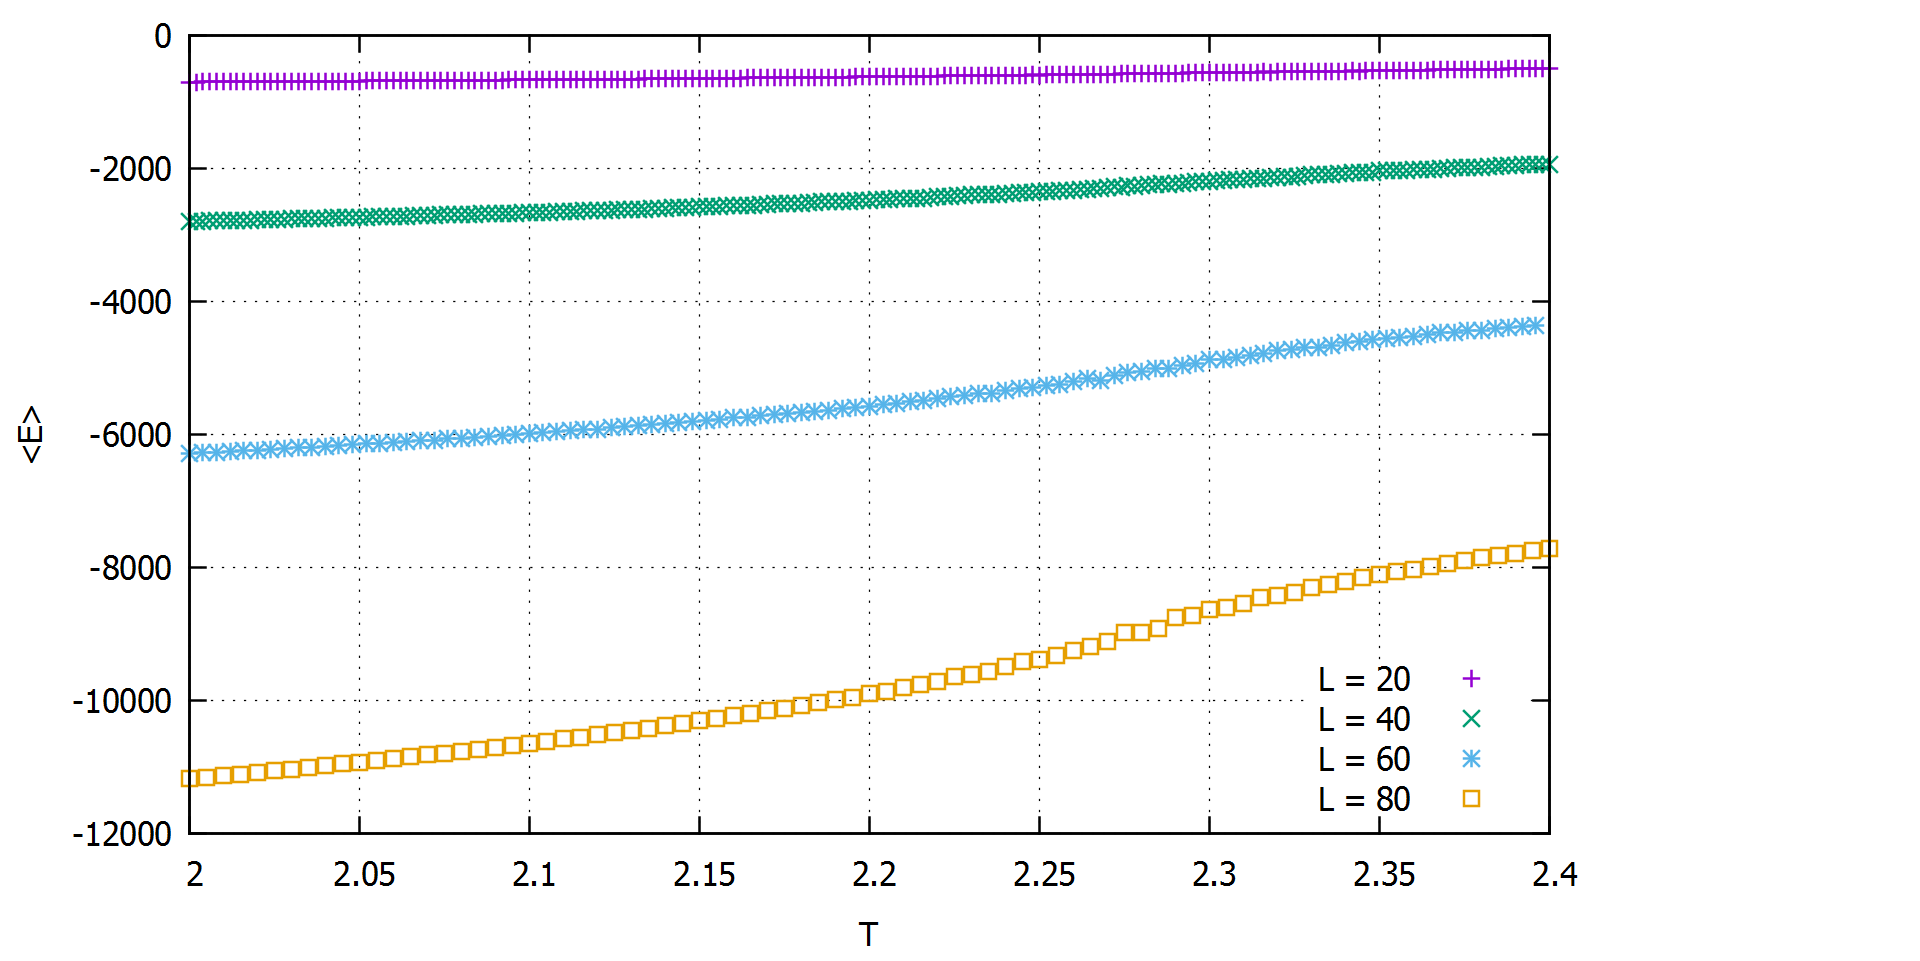
\includegraphics[scale = 0.25]{E_all.png}
	\centering
	\caption{Expectation value of the energy against temperature for different lattice sizes ($10^6$ Monte Carlo cycles)}
	\label{e_all}
\end{figure}

\begin{figure}[h]
	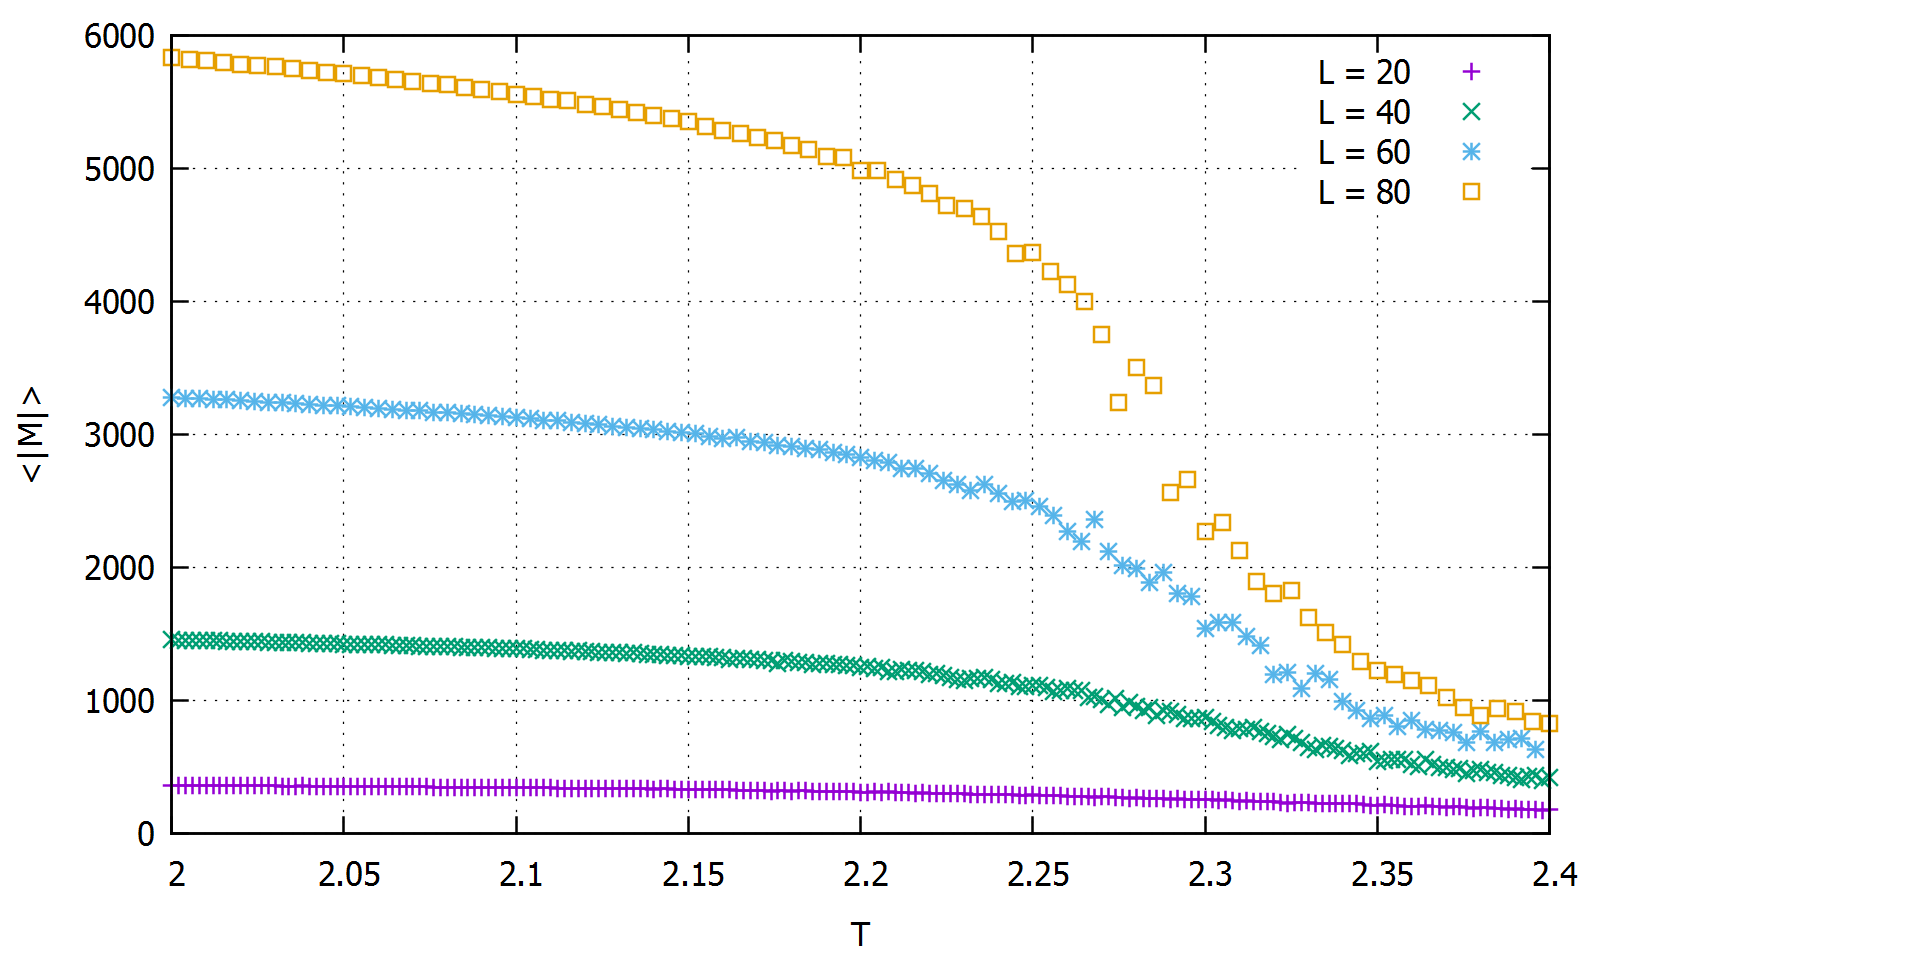
\includegraphics[scale = 0.25]{absm_all.png}
	\centering
	\caption{Expectation value of the absolute magnetisation against temperature for different lattice sizes ($10^6$ Monte Carlo cycles)}
	\label{absm_all}
\end{figure}

\begin{figure}[h]
	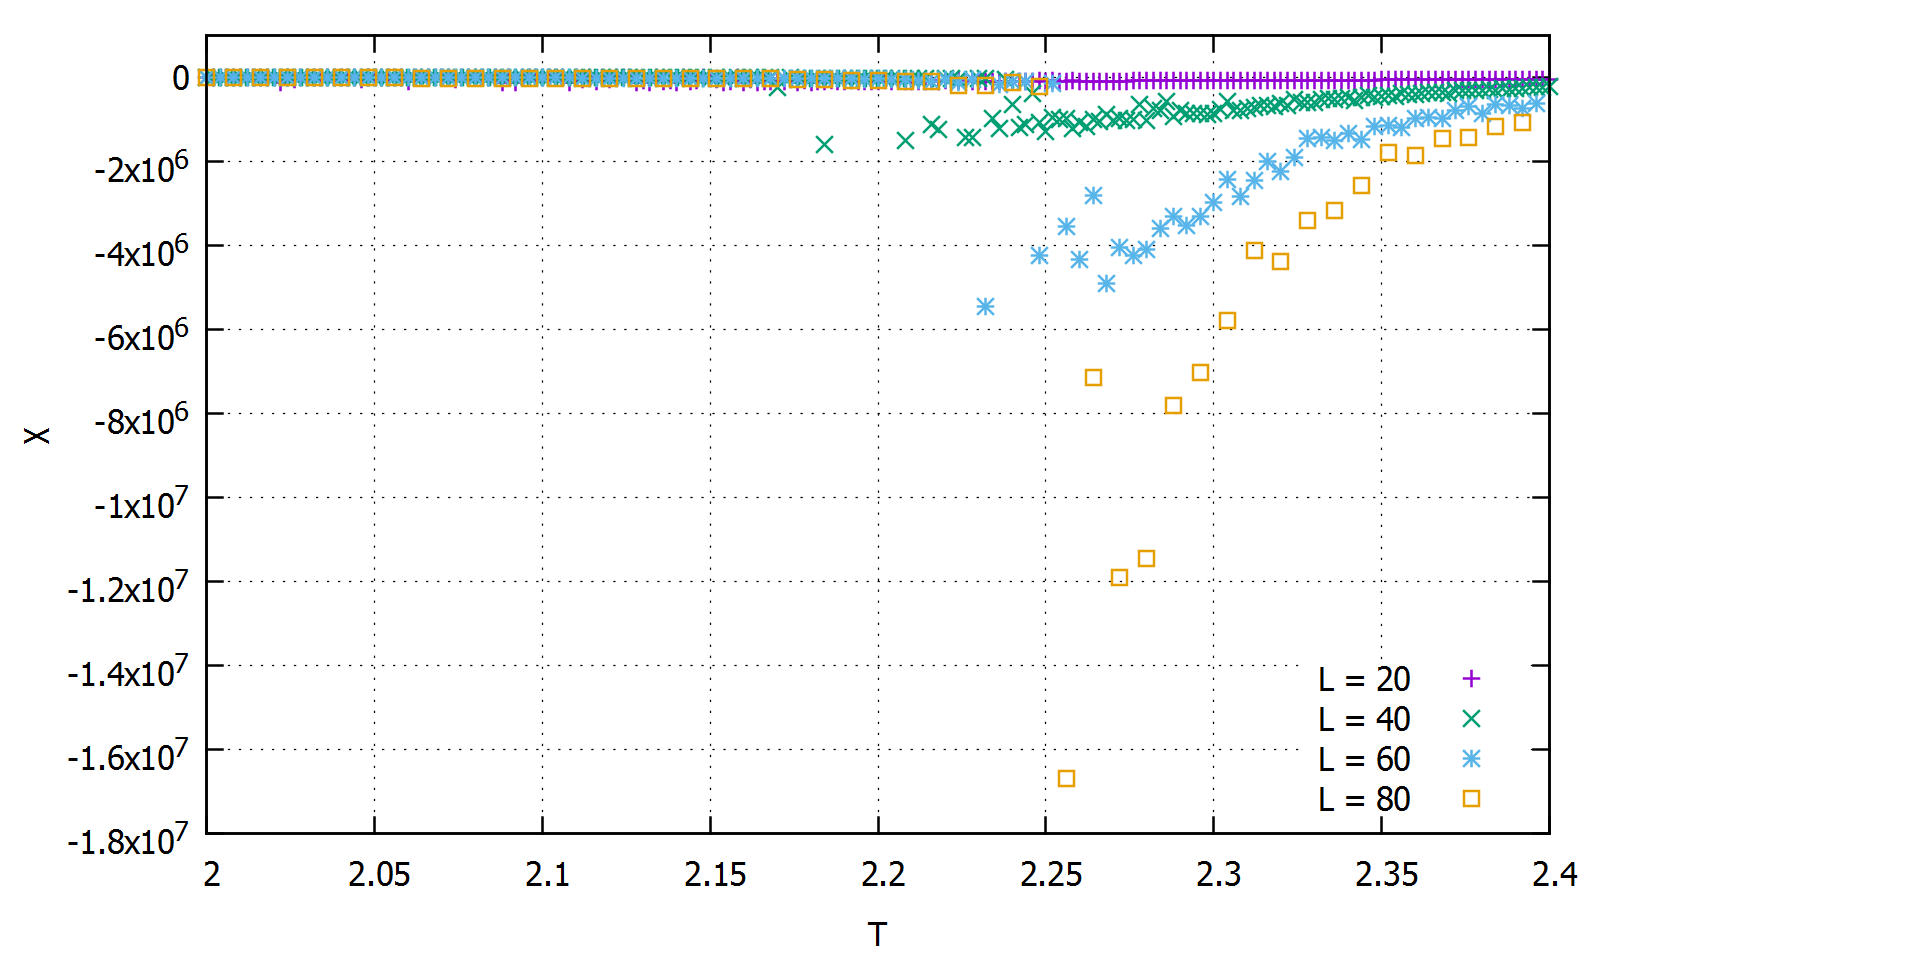
\includegraphics[scale = 0.25]{sus_all.png}
	\centering
	\caption{Susceptibility against temperature for different lattice sizes ($10^6$ Monte Carlo cycles)}
	\label{chi_all}
\end{figure}

\begin{figure}[h]
	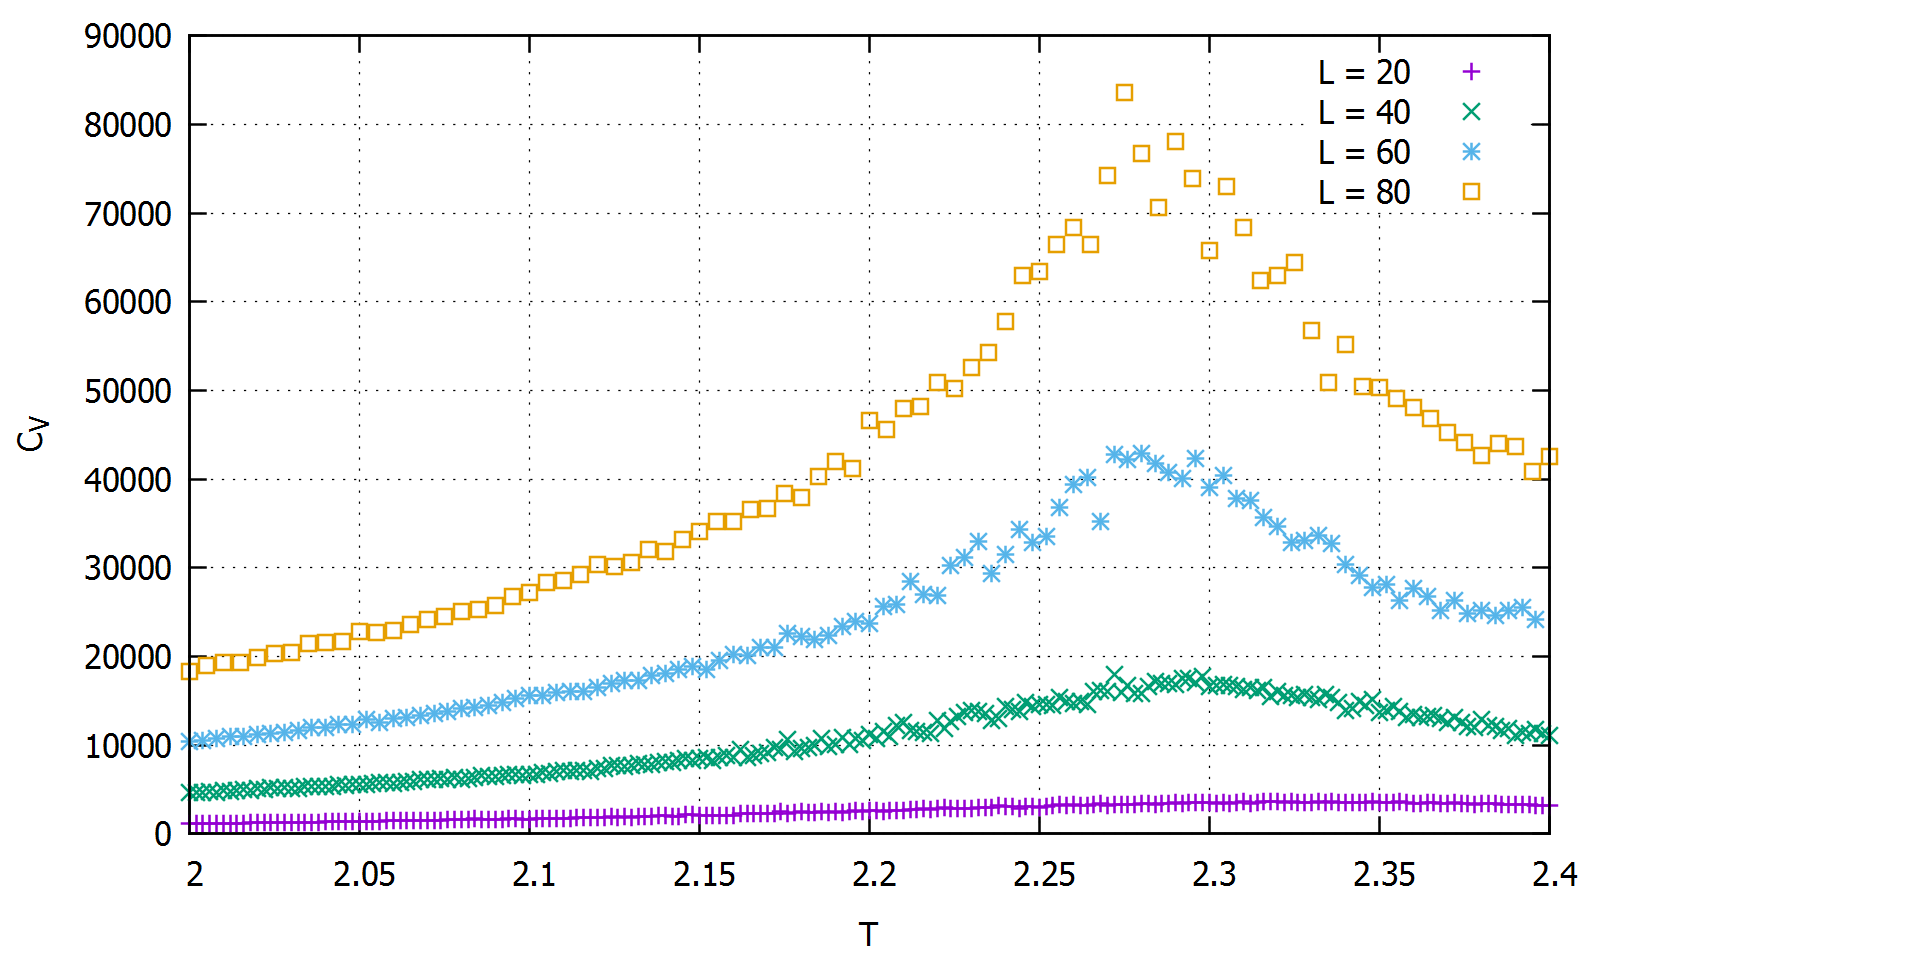
\includegraphics[scale = 0.25]{cv_all.png}
	\centering
	\caption{Expectation value of the specific heat against temperature for different lattice sizes ($10^6$ Monte Carlo cycles)}
	\label{cv_all}
\end{figure}

\begin{figure}[h]
	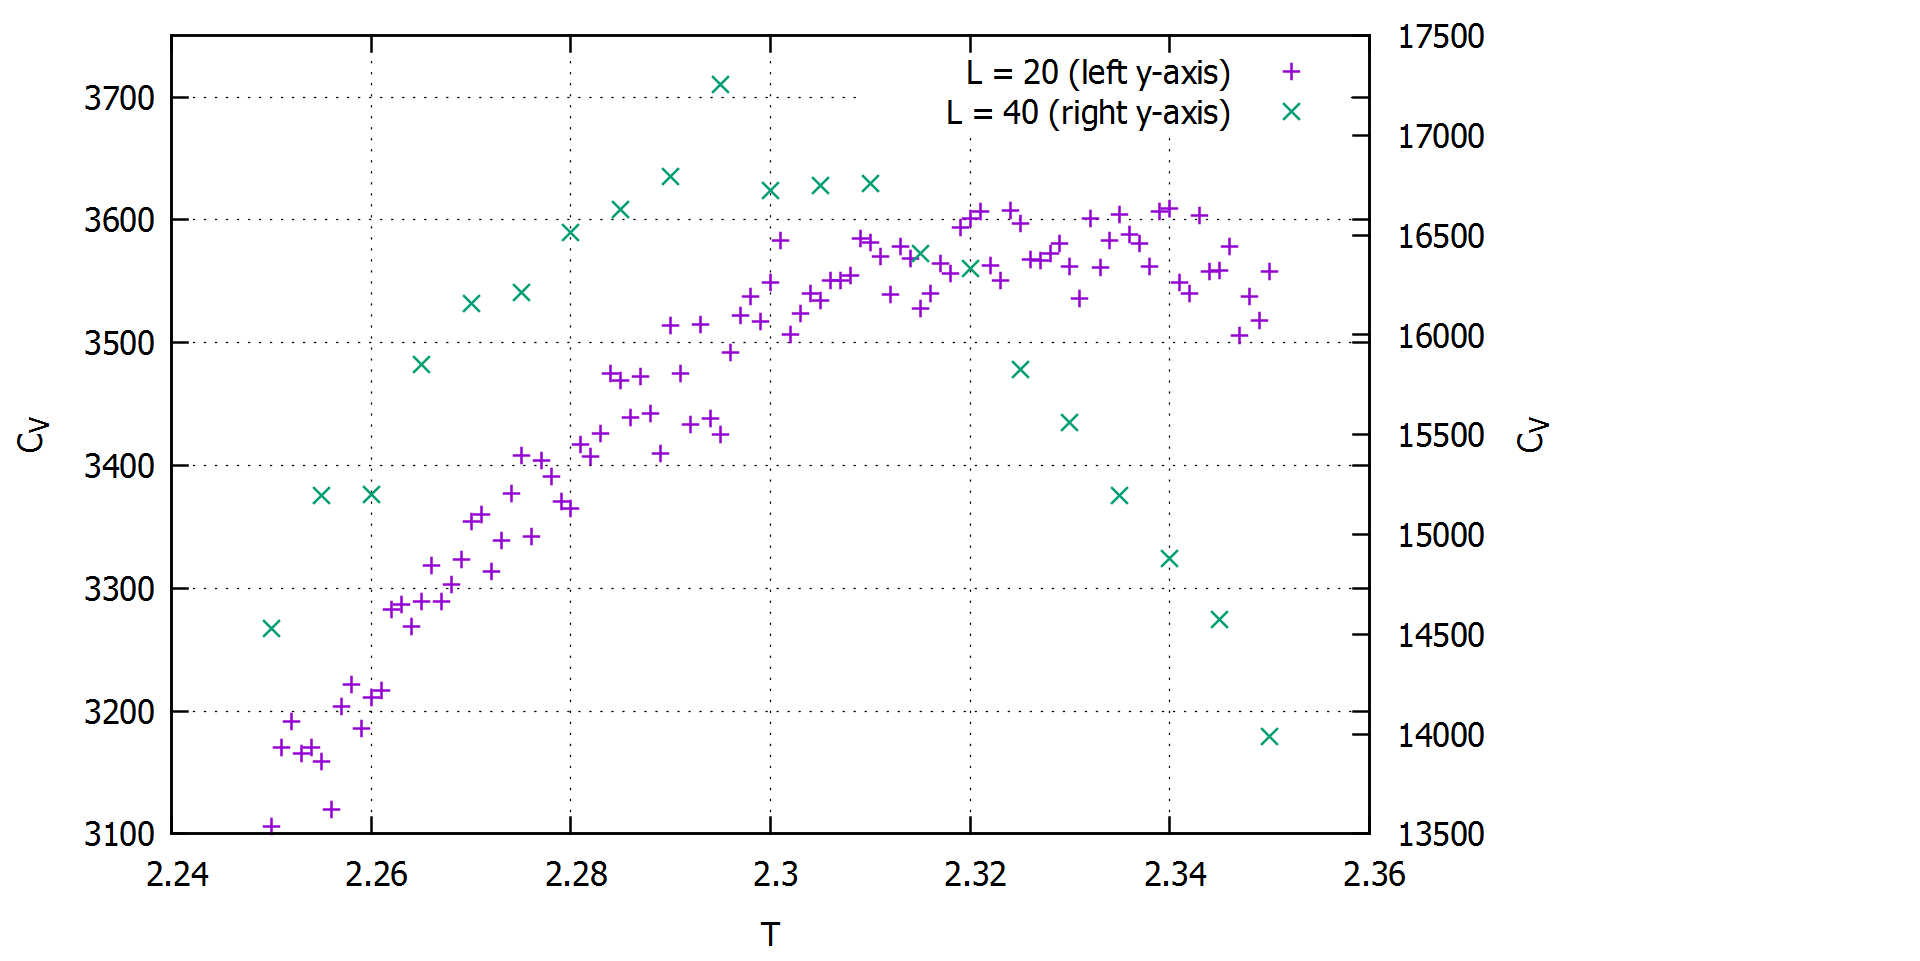
\includegraphics[scale = 0.25]{cv2040.png}
	\centering
	\caption{Expectation value of the specific heat against temperature for lattice sizes L = 20 and L = 40 ($5 \cdot 10^6$ Monte Carlo cycles)}
	\label{cv2040}
\end{figure}

\begin{figure}[h]
	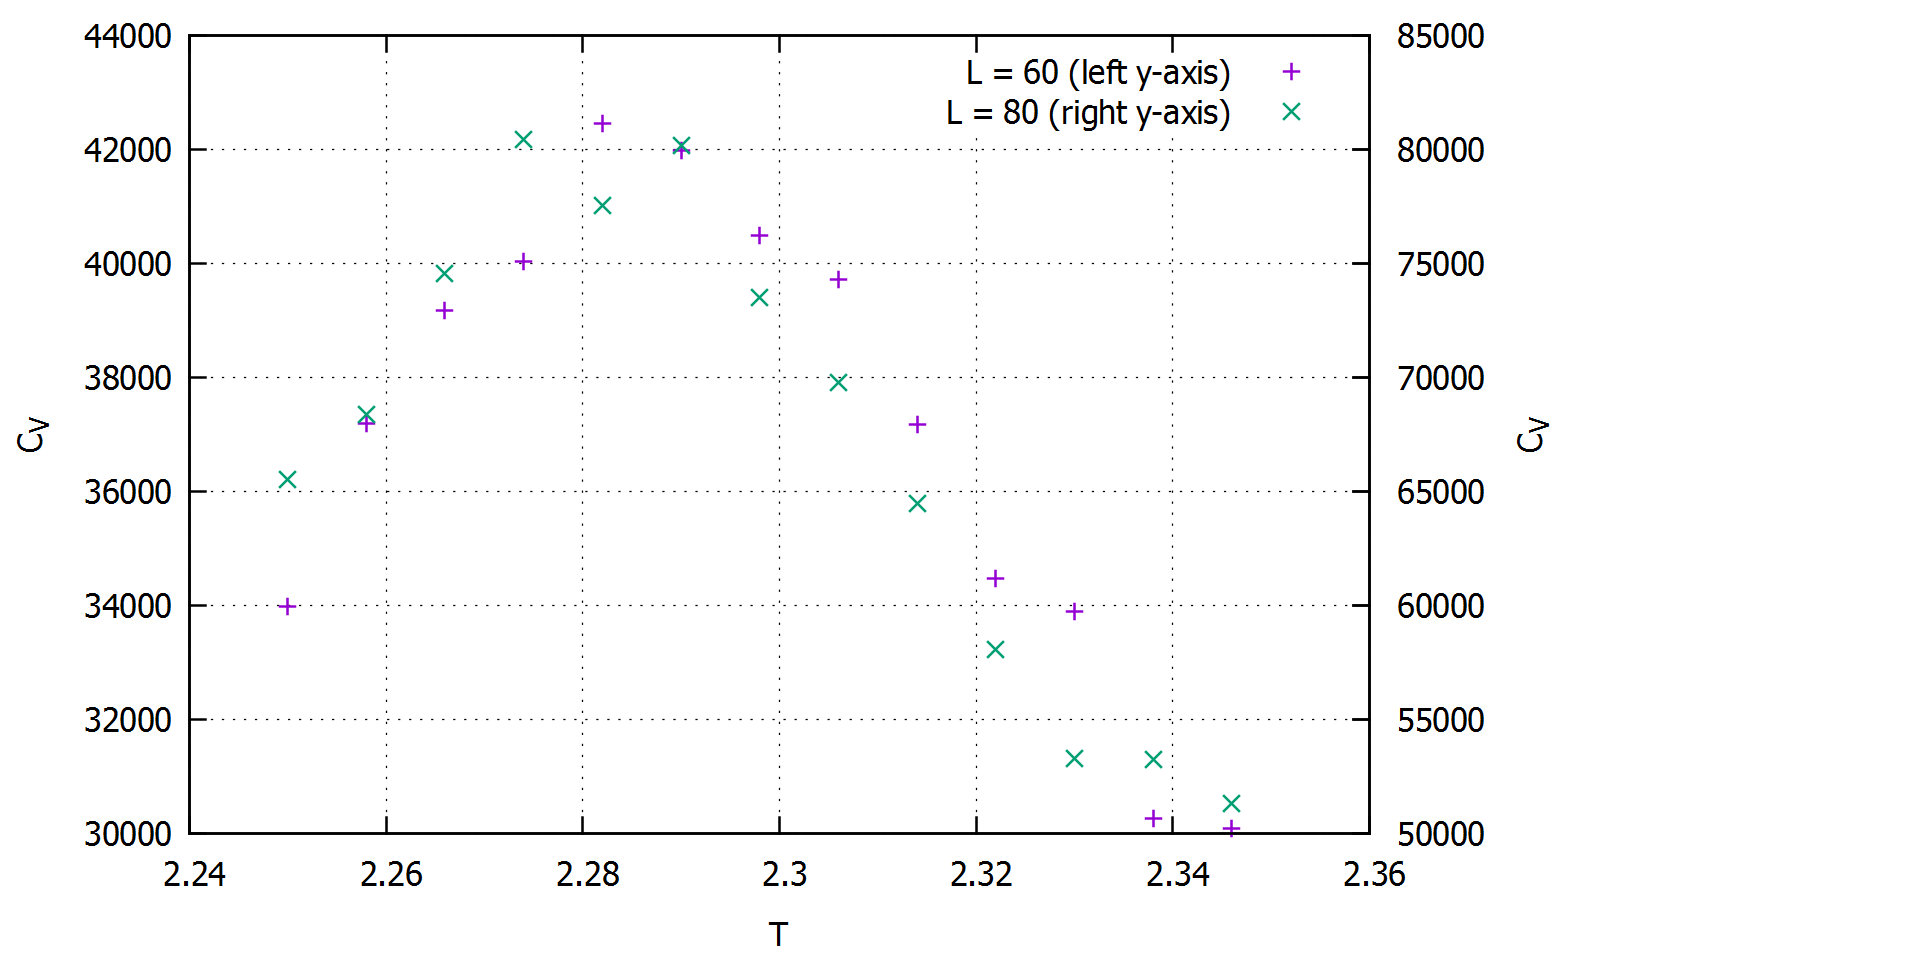
\includegraphics[scale = 0.25]{cv6080.png}
	\centering
	\caption{Expectation value of the specific heat against temperature for lattice sizes L = 60 and L = 80 ($5 \cdot 10^6$ Monte Carlo cycles)}
	\label{cv6080}
\end{figure}

\begin{table}[h!]
	\centering
	\begin{tabular}{|l|r|c|lrp{16cm}}\hline
		L & $T_C$ \\\hline
		20 & $(2.33 \pm 0.01)$\\
		40 & $(2.295 \pm 0.007)$\\
		60 & $(2.285 \pm 0.005)$\\
		80 & $(2.280 \pm 0.007)$\\\hline
	\end{tabular}
	\caption{Critical temperature for different lattice sizes L }
	\label{tc}
\end{table}

\begin{figure}[h]
	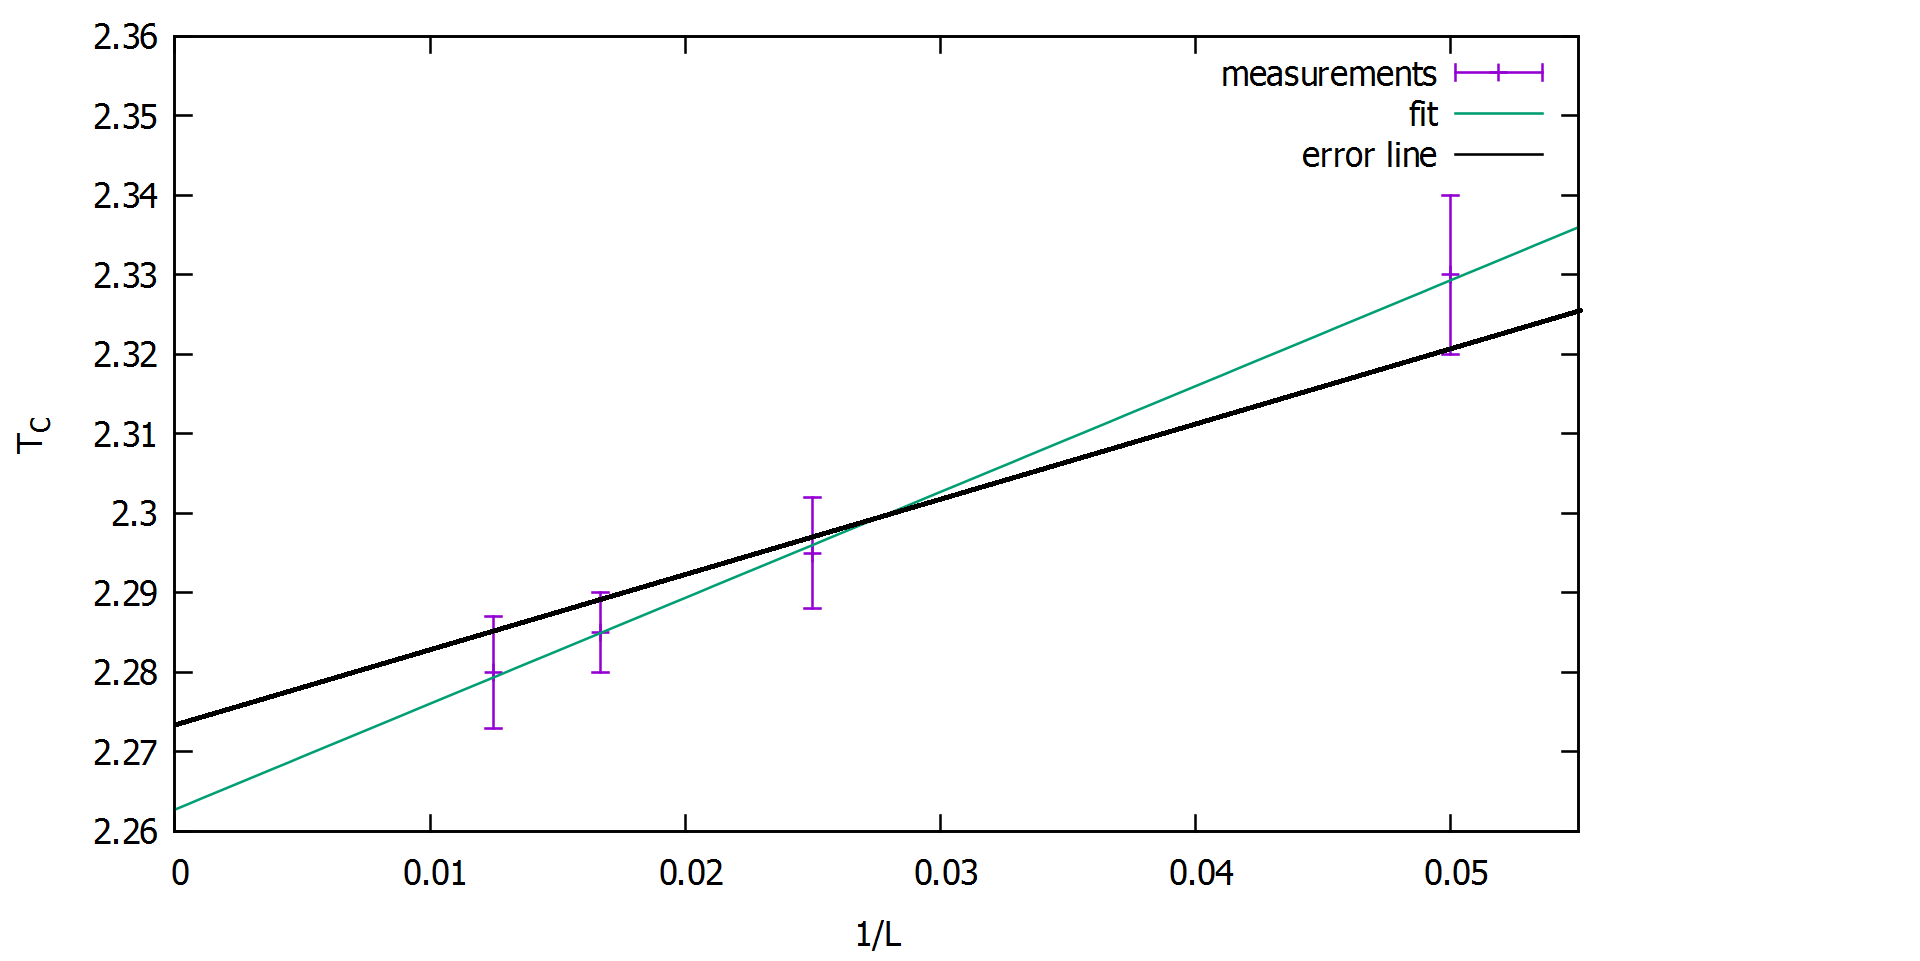
\includegraphics[scale = 0.25]{tc2.png}
	\centering
	\caption{Critical temperature $T_C$ against $\frac{1}{L}$}
	\label{tc2}
\end{figure}


% f part

The connection between different lattice sizes and the critical temperature is given by the following formula

\begin{equation}
T_C(L) - T_C(L = \infty) = a \cdot L^{-\frac{1}{\nu}}
\end{equation}

We have $\nu = 1$, so we get

\begin{equation}
T_C(L) = T_C(L = \infty) + a \cdot \frac{1}{L}
\end{equation}

If we now plot $T_C$ against $\frac{1}{L}$ we should get a line. By measuring the value at which the line crosses the y-axis we can determine $T_C(L = \infty)$. At figure \ref*{tc2} we have plotted our measured values for the critical temperature (which can be seen in table \ref*{tc}) against $\frac{1}{L}$ and signed in a fit line and an error line. The fit line crosses the y-axis at $T_C = 2.263$ while the error line crosses it at $T_C = 2.273$. Thus our value for the critical temperature for an infinite sized lattice is $T_C(L = \infty) = (2.26 \pm 0.01)$. The analytical solution $T_C^{a} = 2.269$ is in the first error interval of this value. Hence our value and the analytical solution match.



\end{document}